\section{Exact reproducible computations}\label{sec:computations}

The computations check the formulas and constructions, compare independently
implemented exact methods, and illustrate the cost of grid restriction. They
use rational arithmetic throughout optimization and verification. Floating
point is used only for plotting and elapsed-time reporting. The supplied
verification bundle records source hashes, exact certificate data, input
transformations, complete rational table values, and all timing samples.
The computer-assisted theorems depend on the exact certificate checks described
in Sections~\ref{sec:reach-four} and~\ref{sec:floor-chambers}; the experiments
below do not substitute for those universal proofs.

\subsection{A pinned public relaxed-control profile}

We use the three-mode Lotka--Volterra relaxed-control profile distributed with
\texttt{pycombina}~\cite{pycombina-data}: 12,000 cells of width $10^{-3}$ on
$[0,12]$. The script retrieves a fixed commit, verifies its SHA-256 digest,
and reads the published decimal entries as rationals. On each cell, it first
normalizes the three nonnegative rates to sum to one, then applies largest
remainder rounding with denominator $10^6$, breaking equal remainders by mode
index. The maximum rate change in the normalization step is less than
$4.959\cdot10^{-7}$. Quantization changes each normalized rate by less than
$10^{-6}$ and therefore changes cumulative allocations by less than
\[
 \delta=12\cdot10^{-6}.
\]
All exact optima reported here concern this quantized piecewise-constant input.
Proposition~\ref{prop:compactness} bounds the change of each optimum relative
to the normalized decimal source by $\delta$. The unnormalized decimal
columns are not taken as simplex-valued input.

The exact one-switch optimum on all 12,000 cells is $1.889$, attained by
switching from mode two to mode three at time $1.889$. A separate enumeration
of every ordered mode pair and every allowed boundary gives the same value.
Direct evaluation at every original input endpoint verifies the returned
schedule. The continuous one-switch optimum for the same input is
\begin{equation}\label{eq:public-continuous}
 \OPT_1(A)=\frac{4721469}{2500000}=1.8885876,
 \qquad \tau=1.8885876,
\end{equation}
with the same mode order. To certify this value, the script locates the unique
crossing of $t-A_p(t)$ and $T-m_q-t$ for each of the six ordered pairs,
using the exact affine formula in its input cell. Their maximum is minimized
at that crossing; the omitted terminal mass is constant. The three-term
formula therefore certifies all pair minima and their global minimum.
Constants are included as endpoint choices. A second evaluation at all input
knots and at the chosen switch verifies the attained error independently.
The fine-grid gap is $1031/2500000=0.0004124$, below the one-switch half-mesh
bound $0.0005$.

\begin{table}[tb]
\centering\small
\caption{Exact quantized public-profile optima on specified uniform switching
grids. All displayed decimals terminate and are exact. Every row uses one
fixed grid for all four budgets; the original input is integrated exactly.}
\label{tab:public-profile}
\begin{tabular}{@{}rrrrrr@{}}
\toprule
Allowed cells $M$ & Width $h$ & $s=0$ & $s=1$ & $s=2$ & $s=3$\\
\midrule
12 & 1 & 3.7771752 & 1.9999996 & 1.8540056 & 0.8540056 \\
24 & 0.5 & 3.7771752 & 1.9999996 & 1.5 & 0.5263358 \\
48 & 0.25 & 3.7771752 & 1.9999996 & 1.5 & 0.52633545
\\
\bottomrule
\end{tabular}
\end{table}

Table~\ref{tab:public-profile} compares budgets on common coarser grids. Their
boundaries are contained in the 12,000-cell grid. Coarse cell masses are exact
sums of the fine masses, and every output schedule is expanded to the original
grid and checked there. Independent labeled-word and boundary enumeration
also verifies every entry for $M=12,24$. The $M=48$ entries are computed by the
exact subset algorithm; its general correctness is established in
Theorem~\ref{thm:fixed-budget}. Increasing the budget on each fixed grid lowers
the optimum. With three switches, refining from 12 to 24 cells gives a much
larger improvement than refining from 24 to 48 cells. These are input-specific
observations, not universal rates or comparisons with a solver using a
different budget.

\begin{table}[tb]
\centering\small
\caption{Certified intervals for both the continuous optimum and the
12,000-cell optimum of the quantized public input. Each interval uses only its
own coarse optimum and the general width-$h$ certificate. Parentheses indicate
a strict lower endpoint.}
\label{tab:public-certificates}
\begin{tabular}{@{}rcc@{}}
\toprule
Allowed cells $M$ & Two switches & Three switches\\
\midrule
12 & $(0.8540056,\,1.8540056]$ & $[0,\,0.8540056]$ \\
24 & $(1,\,1.5]$ & $(0.0263358,\,0.5263358]$ \\
48 & $(1.25,\,1.5]$ & $(0.27633545,\,0.52633545]$
\\
\bottomrule
\end{tabular}
\end{table}

The intervals in Table~\ref{tab:public-certificates} follow from
Theorem~\ref{thm:certified-coarsening}. To certify the normalized decimal source
instead, subtract $\delta$ from each unclipped lower endpoint, add $\delta$
to the upper endpoint, and then clip a negative lower bound to zero. The
returned schedule's error for that source is bounded by the enlarged upper
endpoint. The one-switch rows admit the stronger non-strict lower bound
$U_h-h/2$; with no switches the grid optimum is already the continuous optimum.
Thus these special cases do not need the more conservative general interval.

\subsection{An exactly known continuous comparison}

For the uniform three-mode input on $[0,1]$ with two switches, the continuous
instance optimum equals $1/6$. Here is a direct proof, since
Theorem~\ref{thm:uniform} assumes $k<n$. Omitting a mode incurs error at least
$1/3$. Otherwise all three modes occur once. If the last mode starts at $v$,
its start and final errors imply
\[
 E\ge\max\{v/3,\,2/3-v\}\ge1/6.
\]
The word $(1,2,3)$ with switches at $1/4$ and $1/2$ attains $1/6$ by endpoint
evaluation. Figure~\ref{fig:computations} compares this exact value with coarse
optima for $M=3,4,5,6,8,9,12,16,24$ and their certified lower endpoints.
Each finite-grid optimum is corroborated by separate labeled-word and
boundary enumeration, and the returned schedule is checked directly.
The coarse optima need not decrease between nonnested grids: $M=4$ attains
$1/6$, whereas $M=5$ gives $1/5$. The certificate remains valid on every grid.

\begin{figure}[tb]
\centering
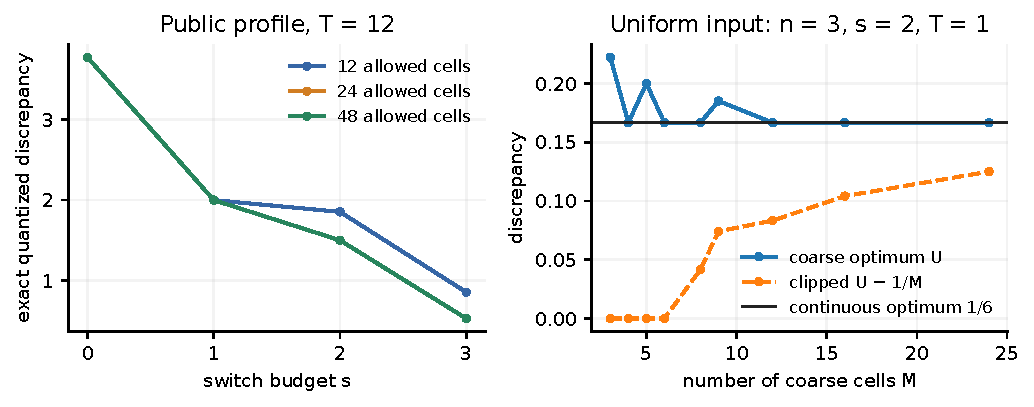
\includegraphics[width=\linewidth]{figures/exact-computations.pdf}
\caption{Left: exact optima on three nested switching grids for the same
quantized public input. Right: coarse upper and clipped lower certificates
for a uniform input with independently known continuous optimum. Lines join
the displayed discrete cases only.}
\label{fig:computations}
\end{figure}

\subsection{Controlled timings and implementation scope}

\newcommand{\FineWall}{0.249}
\newcommand{\FineCPU}{0.246}
\newcommand{\BudgetThreeTwelve}{0.085}
\newcommand{\BudgetThreeTwentyFour}{0.833}
\newcommand{\BudgetThreeFortyEight}{7.980}

Timings use Python 3.13.11 and exact \texttt{Fraction} arithmetic on an Intel
Xeon w5-2565X, Linux under WSL2. Each reported number is the median of three
calls in one process. Inputs are prepared before the timer starts; validation
inside the solver is included, and independent verification afterward is
excluded. Both CPU and wall times and all individual samples are archived.
The host is shared, with no processor affinity or frequency control. These
measurements describe this implementation and workload rather than a general
performance ordering. The full 12,000-cell one-switch solve takes
\FineCPU{} seconds of CPU time and \FineWall{} seconds of wall time.
The three-switch coarse solves take \BudgetThreeTwelve{},
\BudgetThreeTwentyFour{}, and \BudgetThreeFortyEight{} seconds of wall time
for $M=12,24,48$, respectively.

\begin{table}[tb]
\centering\small
\caption{Matched exact methods on deterministic rational inputs. Both methods
optimize the same grid and switch budget. Times are medians in milliseconds;
``words'' counts all labeled-word/boundary cases, including repeated labels.}
\label{tab:controlled-timing}
\begin{tabular}{@{}rrrrrrrr@{}}
\toprule
& & & & \multicolumn{2}{c}{Subset DP} & \multicolumn{2}{c}{Word enumeration}\\
$n$ & $N$ & $s$ & Words & CPU & Wall & CPU & Wall\\
\midrule
3 & 8 & 2 & 567 & 3.85 & 3.82 & 7.48 & 7.42 \\
4 & 8 & 2 & 1344 & 6.67 & 6.62 & 25.44 & 25.25 \\
3 & 8 & 3 & 2835 & 14.02 & 13.92 & 47.71 & 47.36
\\
\bottomrule
\end{tabular}
\end{table}

For Table~\ref{tab:controlled-timing}, cell $j=0,\ldots,N-1$ has width $1/N$
and rates proportional to
$1+((j+2)(i+3)+i^2\bmod 11)$ for $i=0,\ldots,n-1$. Both methods use exact
rationals, and every optimum agrees. The word enumerator computes endpoint
errors independently rather than calling the subset-cost routine.
This is a controlled comparison with exhaustive enumeration, not with SCARP,
\texttt{pycombina}, or the dwell-constrained heuristic in~\cite{abbasi2025}.

\begin{table}[tb]
\centering\small
\caption{Fixed-budget scaling cases: uniform inputs, horizon one, two switches.
The first four rows vary modes at $N=12$; the remaining rows extend the
$n=8$ grid-size comparison. Times are medians in milliseconds.}
\label{tab:scaling-timing}
\begin{tabular}{@{}rrrr@{}}
\toprule
Modes $n$ & Cells $N$ & CPU & Wall\\
\midrule
4 & 12 & 12.38 & 12.26 \\
8 & 12 & 25.67 & 25.42 \\
16 & 12 & 52.25 & 51.74 \\
32 & 12 & 106.19 & 105.15 \\
8 & 8 & 11.35 & 11.24 \\
8 & 16 & 47.39 & 46.92 \\
8 & 24 & 117.75 & 116.65
\\
\bottomrule
\end{tabular}
\end{table}

Table~\ref{tab:scaling-timing} illustrates the separate mode and grid costs at
fixed budget. The $O(nN^2)$ arithmetic bound for two switches is proved in
Section~\ref{sec:algorithms}; a small timing table cannot establish an
asymptotic complexity claim. Rational bit lengths and interpreter overhead
also affect these measurements. Higher budgets increase the boundary
combinations substantially, which is the reason for using a coarse grid with
an explicit accuracy certificate. The experiments do not solve the underlying
nonlinear Lotka--Volterra optimization problem or measure its trajectory,
objective, or path-constraint performance.
